\chapter{Introduction}

\section{Outline of the game}
\begin{figure}[htp]
\centering
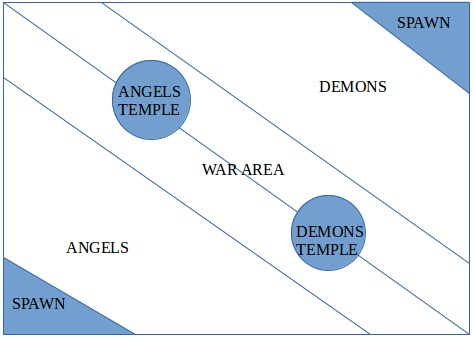
\includegraphics[width=0.7\textwidth]{outline.jpg}
\caption{\label{fig:outline}Bare outline of the map}
\end{figure}


\begin{enumerate}
\item Our game revolves around two teams Angels and Demons.

\item Each team will have its own team area on either side of the diagonal as shown in Figure. 1. The other team is not allowed to enter this area.

\item There is a common war area around the diagonal that both teams are allowed to enter.

\item The common war area around the diagonal will also have strategically located temples for each team.

\item There are 2 players per team. Therefore in total four players are allowed in MultiPlayer mode of the game.

\item The enemy team's team area is never visible.

\item The team's health is represented by the temple's health in the game. Destroying the enemy's temple means reducing enemy temple's health to zero.

\item Each player is assigned a hero. Each hero has his own health. Killing a hero means reducing it's health to zero. A hero is reborn after death in the team’s spawn area.

\item A team's temple health is considerably greater than it's individual hero's health.

\item The team area and war area will have obstacles(stones/trees) located. The hero will have to find paths around these obstacles to their target locations.

\item Each hero is allowed to move in horizontal and vertical direction. Once a target location is identified, the hero will use A* to reach the destination based on above restrictions.

\item The hero while traversing can pick certain items which add to its capabilities. The items are further described in the document.

\item Each hero will have a basic attacking capability and a magic power. Thus, each hero will have two modes of attack : Basic mode and Magic mode. Heros are further described in the document.

\item Each team will have it's own spawn area. A hero when born/re-born will find itself in this spawn area. Hero's can refuel their health by traversing back to this spawn area.
\end{enumerate}


\section{Play Modes}

We plan to offer two play modes for the end user. One being the \textbf{Bot Mode}, and other being the \textbf{MultiPlayer Mode}. In the \textbf{Bot Mode}, there will be one player with three AI players. The \textbf{MultiPlayer Mode} will allow four players on different nodes to play together, two players on each team.








